\section{Experiments}
\label{sec:experiments}

\subsection{Setup} 
\label{sec:exp_setup}
We evaluate 10+ models with non-uniform per-task coverage; the headline figures (Fig.~\ref{fig:main_results}) report seven frontier proprietary systems with full four-task coverage --- \textbf{GPT-4o}, \textbf{GPT-5.3} (think / non-think), \textbf{Claude Opus 4.7} (think / non-think), \textbf{Gemini 3.1 Pro} (think / non-think) --- with open-source baselines (Qwen2.5-VL, InternVL3) and CAD-specialised cadrille-RL on subsets.
For each task, we include a \emph{blind baseline} and evaluate model capabilities by quantifying the performance gains of each model over the baseline across all relevant metrics.
%Inference at temperature 0 with a 60\,s per-sample budget; open models on 8$\times$A800-80GB, proprietary via API.
%We include a \emph{blind baseline} and an \emph{Oracle} reference (GT-code parameter substitution; trivially 100\%).
%Headline numbers use BenchCAD (530 stratified samples); per-model per-task coverage and the full 17{,}900-set scores for the top systems are in Appendix~\ref{app:full_results}.

\subsection{Main Results}
\label{sec:exp_main}

\begin{wrapfigure}{r}{0.5\linewidth} % r=right, width=50% of line
  \vspace{-20pt} % 可选：微调与上方文字的间距
  \centering
  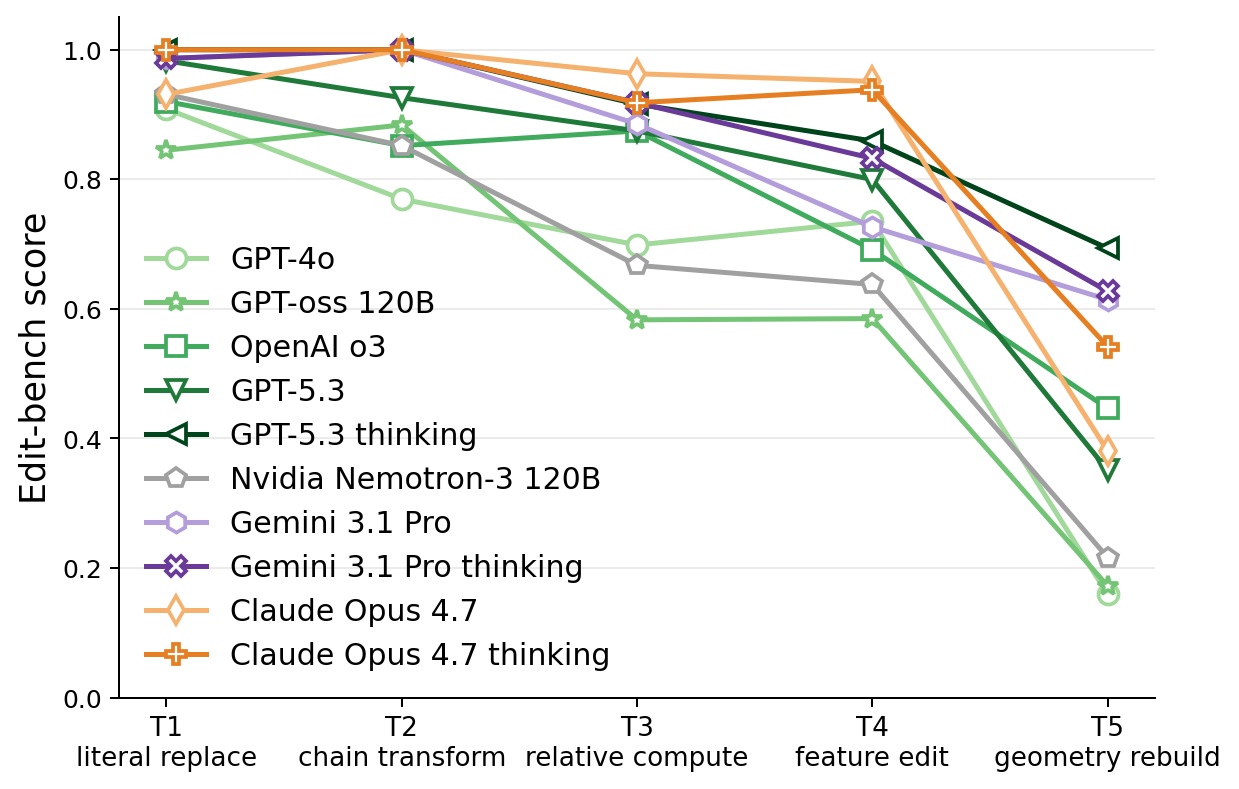
\includegraphics[width=0.9\linewidth]{figures/fig_5.png}
  \caption{\textbf{BenchCAD-Edit by task type.} }
  \label{fig:edit_task}
  \vspace{-10pt} % 可选：微调与下方文字的间距
\end{wrapfigure}

Table~\ref{tab:main_eval_qa_img} indicates that Vision QA remains challenging for current frontier MLLMs. Performance is relatively stronger on Holistic Visual Recognition and Spatial / Code Reasoning, but consistently weaker on CAD Operation Understanding and Industrial Parametric Abstraction, suggesting that models can often recognize global shapes while still struggling to infer CAD operations and parametric design intent. Moreover, thinking mode does not consistently improve performance, because extended reasoning can amplify hallucinations about geometric structures, dimensions, or CAD operations. These results suggest that CAD QA requires more than generic reasoning ability; it demands precise visual grounding, CAD-specific knowledge, and robust parametric abstraction.





Table~\ref{tab:main_eval_qa_code} shows that direct access to CadQuery code substantially improves QA performance compared with the vision-conditioned setting in Table~\ref{tab:main_eval_qa_img}.
The best models achieve total scores around 0.84, far above the best visual-conditioned score of 0.587. 
This large modality gap suggests that current MLLMs are considerably better at extracting geometric and parametric information from explicit CAD programs than from rendered images. 
However, performance on Spatial / Code Reasoning remains comparatively lower, indicating that code access alone does not fully resolve the need for precise spatial and operational reasoning.

The Vision2Code leaderboard (Table~\ref{tab:codegen_unified}) shows three patterns:
(i) the specialist CAD lineage transferred from DeepCAD scores poorly on BenchCAD (Cadrille-RL total 0.338, CADEvolve v3 0.601);
(ii) frontier MLLMs cap mid-range (gemini-3.1-pro-thinking total 0.318) and exhibit non-monotonic thinking-mode behaviour;
(iii) our open Qwen3-VL-2B trained on BenchCAD reaches total 0.628 (iid-sft) and 0.723 (ood-sft$+$RL, best overall) --- showing the dataset is learnable on a small backbone and that RL meaningfully closes the generalisation gap.

\begin{table}[t]
\centering
\small
\setlength{\tabcolsep}{6pt}
\renewcommand{\arraystretch}{1.05}
\caption{\textbf{Vision2Code unified leaderboard.} Specialist CAD lineage (cadrille / CADEvolve), frontier MLLMs, and our open Qwen3-VL-2B trained baseline. All BenchCAD scores on BenchCAD-Lite. \emph{(\,$\dagger$\,)} Ours-SFT-IID is evaluated on the IID split (all 106 families seen at train time); all other rows are OOD on BenchCAD by construction (specialist lineage and frontier MLLMs never saw BenchCAD; ours-SFT-OOD / +RL hold out 10 mech.-transmission families). Essential-op recall is the fraction of ground-truth essential operations (helix / sweep / loft / twist-extrude / parametric involute-gear) recovered by the prediction.}
\label{tab:codegen_unified}
\begin{tabular}{@{}lcccl@{}}
\toprule
Model                                                  & DeepCAD IoU      & BenchCAD IoU            & Ess.\ op recall  & Notes \\
\midrule
\multicolumn{5}{l}{\emph{Specialist CAD lineage ($\sim$2B, OOD on BenchCAD)}} \\
cadrille-RL~\citep{Kolodiazhnyi2026}                   & 0.919            & 0.273                   & --               & sketch+ext, 1M \\
CADEvolve~\citep{Elistratov2026}                       & 0.923            & 0.039                   & --               & extended, 2.7M \\
\midrule
\multicolumn{5}{l}{\emph{Frontier MLLMs (BenchCAD-Lite, by def.\ OOD)}} \\
gpt-4o                                                 & --               & 0.188                   & 0.468            & \\
gpt-5.3 (thinking)                                     & --               & 0.207                   & 0.455            & \\
claude-opus-4.7 (thinking)                             & --               & 0.267                   & 0.471            & \\
gemini-3.1-pro (thinking)                              & --               & \textbf{0.279}          & \textbf{0.567}   & strongest frontier \\
\midrule
\multicolumn{5}{l}{\emph{Ours --- Qwen3-VL-2B, 9 GPU-h on $8{\times}$A800-80GB}} \\
SFT (IID, 106 fam.\ seen)$^{\dagger}$                  & --               & \textbf{0.650}          & \textbf{0.950}   & dataset learnable on 2B \\
SFT (OOD, 10 fam.\ held out)                           & --               & 0.180                   & 0.200            & generalisation gap \\
\quad $+$ RL ($r{=}0.2\,\mathrm{ess}{+}0.8\,\mathrm{IoU}$) & --             & 0.350                   & 0.450            & RL partial recovery \\
\bottomrule
\end{tabular}
\end{table}


% Table~\ref{tab:main_eval} reports per-task accuracy and the macro-mean.
% The strongest model overall is GPT-5.3 (think) at 46.8\% Avg --- well below the IoU $\geq 0.99$ verification threshold and leaving substantial room across every task.
% Three observations stand out.
% \textbf{Absolute scores remain low}: even top reasoning models score below 50\% on every task; the strongest open-source VLM (Qwen2.5-VL-72B, 23.5\% Avg) trails the best proprietary system by 23\,pt; CAD-specialised text/point-cloud models (CAD-Coder-7B, CAD-Recode-1.5B) sit between mid-tier proprietary and top-tier open-source on their applicable tasks despite matching the latter on the original DeepCAD benchmark.
% \textbf{Scaling is not enough}: InternVL3 1B$\to$78B raises Avg by only 14.5\,pt over a 78$\times$ parameter expansion; Qwen2.5-VL 7B$\to$72B by only 7.5\,pt.
% \textbf{Geometry-program decoupling}: several mid-tier models (Gemini 3.1 Pro, GPT-4o) achieve respectable IoU on \texttt{img2cq} but mid-tier scores on \texttt{qa\_img}, indicating they recover the outer shape but cannot answer dimensional questions about it.

% tab_main_eval moved to Appendix~\ref{app:full_results}

\begin{figure*}[t]
  \centering
  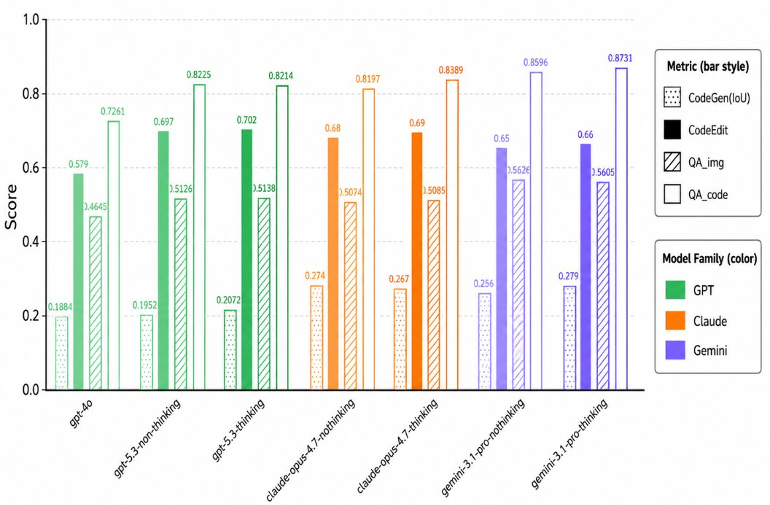
\includegraphics[width=0.65\linewidth]{figures/fig_3.png}
  \caption{\textbf{Per-model performance across the four BenchCAD task categories} (frontier proprietary subset; open-source baselines in Table~\ref{tab:main_eval_qa_img}). Bar style encodes task; colour encodes model family; within-family variants distinguish thinking vs.\ non-thinking. Two patterns motivate the diagnostics that follow: (i) QA-img is consistently lower than QA-code (\emph{Holistic Spatial and Detailing Deficit}, \S\ref{sec:exp_failure_analysis}), and (ii) CodeEdit trails CodeGen on every model, reflecting \emph{Industrial Common Sense Gap} (\S\ref{sec:exp_edit}).}
  \label{fig:main_results}
\end{figure*}


\subsection{Failure Analysis}
\label{sec:exp_failure_analysis}

Building on the layered evaluation introduced in \S\ref{sec:capability}, we examine four representative \textsc{Vision2Code} failures elicited from frontier reasoning models on hard-tier families, each diagnostic of a different level in the capability hierarchy.

\textbf{$L_1$ --- holistic feature recognition.} A hex-head bolt is reproduced with the correct overall body but with its threaded shank and DIN-standard head detail omitted. The vision encoder integrates the global silhouette while failing to register the high-information local features that distinguish a manufacturable bolt from a smooth pin --- a deficit at the perception layer rather than at code generation.

\textbf{$L_1$ --- spatial understanding.} On a bearing retainer cap, the 24-axis rotation-invariant IoU is substantially higher than the single-axis IoU --- a diagnostic signature that the generated geometry is approximately correct but oriented on the wrong base workplane. Inspecting the emitted code confirms it: the model defaults to the XY plane that dominates its training distribution and fails to recognise that the part is naturally extruded along XZ. This is a perception failure at the spatial-anchoring layer rather than a geometric or symbolic one, and one that no amount of code-side reasoning can recover.

\textbf{$L_2$ --- operation understanding.} A twisted bracket is generated as a flat plate with mounting holes; the requisite twist-extrusion is absent from the emitted program entirely. The model recognises the part outline at $L_1$ but fails to map the visible torsion to the corresponding CAD operation, exposing an Op Vocabulary Gap (\S\ref{app:op_gap_full}) at the operation-understanding layer.

\textbf{$L_3$ --- parametric abstraction.} A coil spring with non-uniform pitch is reproduced as a uniform helix. The model recognises the spring family at $L_1$ and emits a helical sweep at $L_2$, yet flattens the pitch profile from variable to constant --- losing the parametric structure that an engineer would have written explicitly. This is an $L_3$ failure invisible to either $L_1$ or $L_2$ metrics, and it is precisely the class of failure that motivates anchoring BenchCAD families to ISO/DIN/EN/ASME/IEC standards.

These cases illustrate how the layered framework converts \textsc{Vision2Code} failures from a single opaque ``wrong code'' category into level-attributable diagnostics: a model can succeed at $L_1$ yet fail at $L_2$ (the bracket), or succeed at $L_1$ and $L_2$ yet fail at $L_3$ (the spring). Without per-level attribution these distinctions collapse into a single low IoU score, and the corresponding training signal --- which level to strengthen --- is lost.

% \subsection{Holistic Spatial and Detailing Deficit and Capability Profile}
% \label{sec:exp_capability}

% The framework of \S\ref{sec:capability} predicts that the gap between \texttt{qa\_img} and \texttt{qa\_code} on matched prompts isolates $L_1$ (Holistic Visual Recognition) from $L_2$ (CAD Operations Understanding).
% Table~\ref{tab:main_eval_qa_img} shows this gap is large and remarkably consistent: 19.6\,pt for GPT-5.3, 19.8\,pt for Claude Opus 4.7, 16.9\,pt for GPT-4o, 12.9\,pt for Qwen2.5-VL-72B.
% We name this the \textbf{Holistic Spatial and Detailing Deficit}.
% It is robust along three axes: it survives chain-of-thought (reasoning variants show the largest absolute gap), survives view-count augmentation (4$\to$8 views recovers $\leq$1.5\,pt; Appendix~\ref{app:ablation}), and survives parameter scaling within open-source families (the relative gap is preserved as absolute scores collapse).
% These properties suggest the Holistic Spatial and Detailing Deficit is a property of the \emph{representation interface} between vision encoders and language decoders, not of any single model's capacity.

% A per-model capability profile across six axes (surface similarity, local feature accuracy, global geometry, CAD understanding, CAD code robustness, synthesis) and four recurring failure modes (\emph{no industry understanding}, \emph{wrong plane}, \emph{wrong ops}, \emph{no detail}) appear in Appendix~\ref{app:capability_profile} (Figure~\ref{fig:capability_profile}); frontier models occupy structurally different capability shapes (GPT-5.3 leads on CAD understanding and code robustness, Claude Opus 4.7 on local feature accuracy and synthesis, Gemini 3.1 Pro on global geometry), confirming that no single model dominates all axes.

\subsection{The Family Cliff}
\label{sec:exp_cliff}

Table~\ref{tab:family_cliff} stratifies \texttt{img2cq} pass rate by family difficulty tier.
The strongest model collapses by 48\,pt from easy (68\%) to hard (20\%), exhibiting a \textbf{Family Cliff} attributable to two interacting factors: hard-tier families exercise advanced operations (helical sweeps, twist-extrusion, lofted Booleans) that scarcely appear in any prior CAD training corpus, and they enforce non-trivial parametric constraints (gear module--tooth--pitch consistency, spring free-length--turn-count coupling) that no model evaluated reliably preserves.
The cliff persists across architectures: closed-source post-training quality dominates the easy-tier gap (Qwen2.5-VL-72B trails GPT-5.3 by 30\,pt on easy) but converges on hard (15\,pt gap) because both models hover near the floor.

% tab_family_cliff moved to Appendix~\ref{app:full_results}

\subsection{The Edit Task: Verified Parametric Editing}
\label{sec:exp_edit}

\paragraph{Setup.} BenchCAD-Edit comprises 748 verified $(\text{original}, \text{instruction}, \text{target})$ triples balanced across all 106 families and stratified into five task types: T1 \emph{literal\_replace}, T2 \emph{chain\_transform}, T3 \emph{relative\_compute}, T4 \emph{feature\_edit}, T5 \emph{geometry\_rebuild} (Table~\ref{tab:task_taxonomy}, Appendix~\ref{app:edit_protocol}). Targets pass through the same expert-verified construction pipeline used for BenchCAD (\S\ref{sec:dataset}).

\paragraph{Metrics.} For a model prediction with rendered solid $S_g$, original solid $S_o$, and target solid $S_t$, let $\mathrm{IoU}(S_a, S_b)$ denote the voxel intersection-over-union at $64^3$. Over $n$ records (failed executions count as zero IoU) we report four pass@1 metrics:
\begin{align}
\mathrm{exec\_rate} &= \tfrac{1}{n}\textstyle\sum_i \mathbf{1}[\,\text{prediction}_i\ \text{ran}\,], \label{eq:exec}\\
\mathrm{strict\_rate} &= \tfrac{1}{n}\textstyle\sum_i \mathbf{1}[\mathrm{IoU}(S_g^i, S_t^i) \geq 0.99], \label{eq:strict}\\
\mathrm{mean\_iou}   &= \tfrac{1}{n}\textstyle\sum_i \mathrm{IoU}(S_g^i, S_t^i), \label{eq:miou}\\
\mathrm{mean\_norm}  &= \tfrac{1}{|\mathcal{N}|}\textstyle\sum_{i \in \mathcal{N}} \mathrm{clip}\!\left(\tfrac{\mathrm{IoU}(S_g^i, S_t^i) - \mathrm{IoU}(S_o^i, S_t^i)}{1 - \mathrm{IoU}(S_o^i, S_t^i)},\,0,\,1\right), \label{eq:norm}
\end{align}
where $\mathcal{N} = \{i : \mathrm{IoU}(S_o^i, S_t^i) \leq 0.99\}$ excludes degenerate records on which the original is already at the target. \texttt{mean\_norm} is a headroom-normalised improvement: $1$ means the model fully traversed the original-to-target gap, $0$ means it did not move at all. All metrics are pass@1: a single API call per (record, model) with no resampling. A complementary 6-orientation rotation-invariant voxel IoU is computed alongside the standard IoU and used only for failure attribution (\S\ref{sec:exp_failure_analysis}, \emph{wrong-plane} diagnostic).

\paragraph{Models.} We score ten code LLMs spanning 2024--2026: \texttt{gpt-4o} (OpenAI, 2024), \texttt{o3} (OpenAI, 2025), \texttt{gpt-oss-120b} (OpenAI open-weights, 2025), \texttt{gpt-5.3-chat-latest} with and without \texttt{reasoning=medium} (OpenAI, 2025--26), \texttt{nemotron-3-super-120b-a12b} (NVIDIA, 2026), \texttt{gemini-3.1-pro-preview} with and without thinking (Google DeepMind, 2026), and \texttt{claude-opus-4-7} with and without \texttt{reasoning=high} (Anthropic, 2026). Closed models are queried through their official APIs; open-weights models via OpenRouter.


  \paragraph{Findings.} Table~\ref{tab:main_results} ranks the ten models by \texttt{mean\_norm}; Figure~\ref{fig:edit_task} disaggregates performance over T1--T5. Read together they validate three design choices that BenchCAD-Edit makes deliberately, and only secondarily produce a leaderboard.                                                             
  \textbf{The metric: \texttt{mean\_norm} is the principled signal, not \texttt{mean\_iou}.} Because every pair is constructed from a verified non-trivial original ($\mathrm{IoU}_{\mathrm{rot}}(S_o, S_t)$ ranges from     
  $0.10$ to $0.95$ across the 748 pairs), a model that emits the original unchanged already collects substantial \texttt{mean\_iou} on the easier pairs
  --- inflating the headline number without any actual editing.
  \texttt{mean\_iou} is still useful as a \emph{geometric closeness} signal and is reported for completeness, but the quantity that asks \emph{``did the model traverse the original-to-target gap''} is Eq.~\eqref{eq:norm}: the per-pair
  improvement, normalised by the available headroom $(1 - \mathrm{IoU}(S_o, S_t))$, clipped to $[0, 1]$, then averaged. Concretely, \texttt{claude-opus-4-7} (no-thinking) attains the highest \texttt{mean\_iou} of any model at $0.956$ but ranks 4th on \texttt{mean\_norm} ($0.811$) and 4th on \texttt{strict\_rate} ($79.2\%$): high mean IoU buys it nothing once we control for the per-pair starting point. The persistent $5$--$25$\,pt gap between \texttt{strict\_rate} and \texttt{mean\_iou}\,$\times 100$ across every row of Table~\ref{tab:main_results} is the same effect from another
  angle: models routinely produce outputs that are \emph{geometrically close} to the target without satisfying the parametric $\mathrm{IoU} \geq 0.99$ threshold, and only \texttt{mean\_norm} prices this in correctly.

\textbf{The task taxonomy: T1--T5 is what makes the benchmark diagnostic.}    
  Aggregate \texttt{mean\_norm} compresses the leaderboard into a single $0.56$--$0.87$ band; the per-task-type curves in Figure~\ref{fig:edit_task} reveal that this band is the average of qualitatively different regimes. T1 (\emph{literal\_replace}) is saturated at $\geq 0.93$ for every modern model and would fail to discriminate any pair of systems on its own. T2 (\emph{chain\_transform}) preserves the same ordering with a slight spread. The gap opens at T3 (\emph{relative\_compute}): models that solve T1 perfectly
   drop $0.10$--$0.30$\,pt because reading one literal and computing another is a different capability than copying a target value. T4 (\emph{feature\_edit}) introduces another step, separating models that can locate and rewrite a CSG
  sub-block from those that cannot. T5 (\emph{geometry\_rebuild}) collapses every model onto a $0.15$--$0.70$ floor: even the strongest reasoning systems, \texttt{gpt-5.3-thinking} and
  \texttt{claude-opus-4-7-reasoning}, bottom out at $\sim 0.6$ on
  coordinated multi-block restructures with trig-derived geometry. Without the T1--T5 split, the T5 collapse would be invisible. The split is also designed to align with the L1--L4 capability hierarchy used in the failure analysis below: T1 and T2 primarily probe \textbf{L2 (CAD Operations Comprehension)}
  --- the model must locate and emit the right API call, but no parameter reasoning is required; T3 isolates \textbf{L3 (Industrial Parametric Abstraction)} by demanding arithmetic over an existing literal; T4 and T5 require \textbf{L4 (Spatial Reasoning + Code Synthesis)}, composing multiple sub-feature edits in concert. \textbf{L1 (Holistic Visual Understanding)} is a prerequisite for every type, since the model must read the original program correctly before editing it. Higher T-levels accordingly subsume lower-level competence, which is why per-model curves in Figure~\ref{fig:edit_task} are monotone in T-index rather than crossing.

  \textbf{Per-model patterns.} Three patterns emerge once the metric and the task split are fixed. (i) \emph{Reasoning is the strongest single intervention.} For all three vendors that publish a thinking variant, switching it on lifts \texttt{mean\_norm} by $4$--$13$\,pt: \texttt{gpt-5.3-chat-latest} $0.740 \to 0.865$ ($+12.5$), \texttt{claude-opus-4-7} $0.811 \to 0.853$ ($+4.2$), \texttt{gemini-3.1-pro-preview} $0.795 \to 0.837$ ($+4.2$); the three thinking variants occupy ranks 1--3 on the leaderboard. (ii) \emph{Execution rate is uninformative on its own.} \texttt{claude-opus-4-7} (no-think) leads on \texttt{exec\_rate} ($98.4\%$) but trails its thinking sibling by $4.2$\,pt on \texttt{mean\_norm}; running cleanly is necessary, not sufficient. (iii) \emph{Open-weights frontier still trails.} \texttt{nemotron-3-super-120b-a12b} ($0.608$) and \texttt{gpt-oss-120b} ($0.561$) sit at the bottom together with the older closed model \texttt{gpt-4o} ($0.615$); the gap to the closed reasoning frontier is $\sim 25$\,pt, with most of the deficit accumulated past \texttt{mean\_norm}; running cleanly is necessary, not sufficient. (iii)
  \emph{Open-weights frontier still trails.} \texttt{nemotron-3-super-120b-a12b} ($0.608$) and \texttt{gpt-oss-120b} ($0.561$) sit at the bottom together with the older closed model \texttt{gpt-4o} ($0.615$); the gap to the closed
  reasoning frontier is $\sim 25$\,pt, with most of the deficit accumulated past T3. We read this as evidence that BenchCAD-Edit measures something that current open-weights training does not yet target, rather than a verdict on the absolute capability of any single model.

\paragraph{Failure Analysis. Placeholder} A failure-code breakdown (E001--E004 defined in Table~\ref{tab:error_codes}; per-model distribution in Fig.~\ref{fig:edit_error_pies}) shows the dominant failure shifts with model class: \texttt{gpt-4o} and \texttt{gpt-oss-120b} are bottlenecked by \emph{wrong\_operation} (real API, wrong selector or argument), while reasoning-tier models trade hallucinations for \emph{no\_op} edits in which the agent rewrites the original byte-for-byte.

\begin{table}[t]
\centering
\caption{\textbf{BenchCAD-Edit leaderboard.} Code LLMs evaluated on $n \approx 748$ pairs each under the metrics defined in \S\ref{sec:exp_edit} (\texttt{exec\_pct}, \texttt{mean\_iou}, \texttt{mean\_cd}, \texttt{ess\_score}, \texttt{total}). Models ranked by \texttt{total}. \emph{Thinking} indicates the reasoning-mode variant where applicable. Every prediction is a single pass@1 API call. \textcolor{red}{Frontier-model numbers below are placeholders pending the full eval run.}}
\label{tab:main_results}
\small
\setlength{\tabcolsep}{5pt}
\begin{tabular}{@{}rllcccc@{}}
\toprule
\textbf{Rank} & \textbf{Model} & \textbf{Vendor} & \textbf{Thinking} & \textbf{exec\_pct} & \textbf{ess\_score} & \textbf{total} \\
\midrule
-- & GPT-5.3                & OpenAI    & \cmark  & -- & -- & -- \\
-- & Claude Opus 4.7        & Anthropic & \cmark  & -- & -- & -- \\
-- & Gemini 3.1 Pro         & Google    & \cmark  & -- & -- & -- \\
-- & Claude Opus 4.7        & Anthropic & --      & -- & -- & -- \\
-- & Gemini 3.1 Pro         & Google    & --      & -- & -- & -- \\
-- & GPT-5.3                & OpenAI    & --      & -- & -- & -- \\
-- & OpenAI o3              & OpenAI    & \cmark  & -- & -- & -- \\
-- & GPT-4o                 & OpenAI    & --      & -- & -- & -- \\
\bottomrule
\end{tabular}
\end{table}


\subsection{Open BenchCAD-Trained Baseline: Recipe}
\label{sec:exp_training}

For reproducibility we describe the open Qwen3-VL-2B baseline whose scores appear in the bottom block of Table~\ref{tab:codegen_unified}.
\textbf{SFT}: two splits --- IID (all 106 families seen at train time) and OOD (10 mech.-transmission families held out from training, evaluated on those held-out families).
\textbf{RL}: on-policy GRPO-varient from each SFT checkpoint, reward $r{=}0.2\,\mathrm{ess}{+}0.8\,\mathrm{IoU}$ ($r{=}-1$ on parse error / timeout / zero-volume); RL data excludes OOD families; no warm-start. Per-operation recall ablation in Table~\ref{tab:op_gap}; full training configs and curves in Appendix~\ref{app:op_gap_full}.
